\let\negthickspace\undefined
\documentclass[journal,12pt,twocolumn]{IEEEtran}
\usepackage{cite}
\usepackage{amsmath,amssymb,amsfonts,amsthm}
\usepackage{algorithmic}
\usepackage{graphicx}
\usepackage{textcomp}
\usepackage{xcolor}
\usepackage{txfonts}
\usepackage{listings}
\usepackage{enumitem}
\usepackage{mathtools}
\usepackage{gensymb}
\usepackage{comment}
\usepackage[breaklinks=true]{hyperref}
\usepackage{tkz-euclide} 
\usepackage{listings}
\usepackage{gvv}                                        
\def\inputGnumericTable{}                                 
\usepackage[latin1]{inputenc}                                
\usepackage{color}                                            
\usepackage{array}                                            
\usepackage{longtable}                                       
\usepackage{calc}                                             
\usepackage{multirow}                                         
\usepackage{hhline}                                           
\usepackage{ifthen}                                           
\usepackage{lscape}
\usepackage{tfrupee}
\usepackage{ragged2e}

\newtheorem{theorem}{Theorem}[section]
\newtheorem{problem}{Problem}
\newtheorem{proposition}{Proposition}[section]
\newtheorem{lemma}{Lemma}[section]
\newtheorem{corollary}[theorem]{Corollary}
\newtheorem{example}{Example}[section]
\newtheorem{definition}[problem]{Definition}
\newcommand{\BEQA}{\begin{eqnarray}}
\newcommand{\EEQA}{\end{eqnarray}}
\newcommand{\define}{\stackrel{\triangle}{=}}
\theoremstyle{remark}
\newtheorem{rem}{Remark}

\begin{document}

\bibliographystyle{IEEEtran}
\vspace{3cm}

\title{GATE.CH.61}
\author{EE23BTECH11062 - V MANAS}
\maketitle
\newpage

\bigskip
\textbf{Question:}\\The outlet concentration $C_A$ of a plug flow reactor (PFR) is controlled by manipulating the inlet concentration $C_{A0}$.The following transfer function describes the dynamics of this PFR.
\begin{align*}
    \frac{C_{A}(s)}{C_{A0}(s)}=e^{-(\frac{V}{F})(k+s)}
\end{align*}
In the above question, V=1$m^3$,F=0.1$m^3$$min^{-1}$ and k=0.5$min^{-1}$.The measurement and valve transfer functions are both equal to 1.The ultimate gain, defined as the proportional controller gain that produces sustained oscillations, for this system is\\ \hfill{(GATE 2023 CH 61)}\\
\textbf{Solution:}\\
\begin{table}[h]
    \centering
    \begin{tabular}{|c|c|c|c}
    \hline
    \textbf{Variable} & \textbf{Description} & \textbf{Values}\\
    \hline
    $G_o$ & overall transfer function & 1\\
    \hline
    $G_p$ & process transfer function & \\
    \hline
    $G_c$ & proportional controller transfer function & \\
    \hline
    $K_c$ & gain of the proportional controller & \\
    \hline
\end{tabular}

    \caption{Variables Used}
    \label{tab:GATE2023.CH.61}
\end{table}
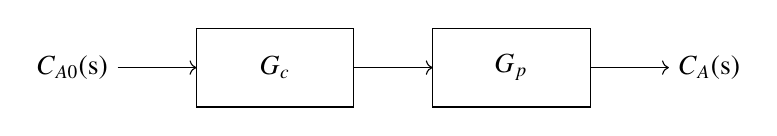
\begin{tikzpicture}
\centering
    % Draw the main box
    \node[draw, minimum width=2cm, minimum height=1cm] (box) at (0,0) {$G_c$};
    \draw[->] (-2,0) -- (-1,0);
    \draw[->] (1,0) -- (2,0);
    \node[anchor=east] at (-2,0) {$C_{A0}$(s)};
    \node[draw, minimum width=2cm, minimum height=1cm] (box) at (3,0) {$G_p$};
    \draw[->] (4,0) -- (5,0);
    \node[anchor=west] at (5,0) {$C_{A}$(s)};
\end{tikzpicture}
\begin{align}
    G(s)&=\frac{C_A(s)}{C_{A0}(s)}=e^{-(\frac{V}{F})(k+s)}\\
    G(s)&=e^{-(\frac{1}{0.1})(0.5+s)}\\
    G(s)&=e^{-(10s+5)}
\end{align}
The transfer function of a proportional controller is $K_c$ so we can take,$G_c$=$K_c$\\
Given that the measurement and valve transfer functions are both equal to 1, we can take $G_p$=G(s)
\begin{align}
    G_o&=G_p\times G_c\\
    G_o&=G(s)\times K_c\\
    1&=e^{-(10s+5)}\times K_C\\
    1&=1\times \frac{K_c}{e^5}
\end{align}
$\therefore K_c=e^5=148.11$
\end{document}
